%% LyX 2.2.0 created this file.  For more info, see http://www.lyx.org/.
%% Do not edit unless you really know what you are doing.
\documentclass[english]{beamer}
\usepackage[T1]{fontenc}
\usepackage[latin9]{inputenc}
\setcounter{secnumdepth}{3}
\setcounter{tocdepth}{3}
\usepackage{babel}
\usepackage{amsmath}
\usepackage{graphicx}
\ifx\hypersetup\undefined
  \AtBeginDocument{%
    \hypersetup{unicode=true,pdfusetitle,
 bookmarks=true,bookmarksnumbered=false,bookmarksopen=false,
 breaklinks=false,pdfborder={0 0 1},backref=false,colorlinks=true}
  }
\else
  \hypersetup{unicode=true,pdfusetitle,
 bookmarks=true,bookmarksnumbered=false,bookmarksopen=false,
 breaklinks=false,pdfborder={0 0 1},backref=false,colorlinks=true}
\fi

\makeatletter

%%%%%%%%%%%%%%%%%%%%%%%%%%%%%% LyX specific LaTeX commands.
%% Because html converters don't know tabularnewline
\providecommand{\tabularnewline}{\\}

%%%%%%%%%%%%%%%%%%%%%%%%%%%%%% Textclass specific LaTeX commands.
 % this default might be overridden by plain title style
 \newcommand\makebeamertitle{\frame{\maketitle}}%
 % (ERT) argument for the TOC
 \AtBeginDocument{%
   \let\origtableofcontents=\tableofcontents
   \def\tableofcontents{\@ifnextchar[{\origtableofcontents}{\gobbletableofcontents}}
   \def\gobbletableofcontents#1{\origtableofcontents}
 }
 \newenvironment{lyxcode}
   {\par\begin{list}{}{
     \setlength{\rightmargin}{\leftmargin}
     \setlength{\listparindent}{0pt}% needed for AMS classes
     \raggedright
     \setlength{\itemsep}{0pt}
     \setlength{\parsep}{0pt}
     \normalfont\ttfamily}%
    \def\{{\char`\{}
    \def\}{\char`\}}
    \def\textasciitilde{\char`\~}
    \item[]}
   {\end{list}}

%%%%%%%%%%%%%%%%%%%%%%%%%%%%%% User specified LaTeX commands.
\usetheme[secheader]{Boadilla}
\usecolortheme{seahorse}
\title[Curry-Howard code generator]{Generating code with the Curry-Howard correspondence}
\subtitle{Type inhabitation at compile time}
\author{Sergei Winitzki}
\date{December 25, 2017}
\institute[ABTB]{Academy by the Bay}
\setbeamertemplate{navigation symbols}{}

\makeatother

\begin{document}
\frame{\titlepage}
\begin{frame}{Types and propositional logic}


\framesubtitle{The Curry-Howard correspondence}

The code \texttt{\textcolor{blue}{\footnotesize{}val x:\ T =}} ...
shows that \emph{we can compute a value} of type \texttt{\textcolor{blue}{\footnotesize{}T}}
as part of our program expression
\begin{itemize}
\item Let's denote this \emph{proposition} by ${\cal CH}(T)$ \textendash{}
``$\mathcal{C}$ode $\mathcal{H}$as a value of type \texttt{\textcolor{blue}{\footnotesize{}T}}''
\item Correspondence between types and propositions, for a given program:
\end{itemize}
\begin{center}
\begin{tabular}{|c|c|c|}
\hline 
\textbf{Type} & \textbf{Proposition} & \textbf{Short notation}\tabularnewline
\hline 
\hline 
\texttt{\textcolor{blue}{\footnotesize{}T}} & ${\cal CH}(T)$ & $T$\tabularnewline
\hline 
\texttt{\textcolor{blue}{\footnotesize{}(A, B)}} & ${\cal CH}(A)$ \emph{and} ${\cal CH}(B)$ & $A\times B$\tabularnewline
\hline 
\texttt{\textcolor{blue}{\footnotesize{}Either{[}A, B{]}}} & ${\cal CH}(A)$ \emph{or} ${\cal CH}(B)$ & $A+B$\tabularnewline
\hline 
\texttt{\textcolor{blue}{\footnotesize{}A $\Rightarrow$ B}} & ${\cal CH}(A)$ \emph{implies} ${\cal CH}(B)$ & $A\Rightarrow B$\tabularnewline
\hline 
\texttt{\textcolor{blue}{\footnotesize{}Unit}} & \emph{True} & 1\tabularnewline
\hline 
\texttt{\textcolor{blue}{\footnotesize{}Nothing}} & \emph{False} & 0\tabularnewline
\hline 
\end{tabular}
\par\end{center}
\begin{itemize}
\item Type parameter \texttt{\textcolor{blue}{\footnotesize{}{[}T{]}}} in
a function type means $\forall T$
\item Example: \texttt{\textcolor{blue}{\footnotesize{}def dupl{[}A{]}:\ A
$\Rightarrow$ (A, A)}}. The type of this function corresponds to
the (valid) theorem $\forall A:A\Rightarrow A\times A$
\end{itemize}
\end{frame}

\begin{frame}{The CH correspondence: proposition$\rightarrow$type / proof$\rightarrow$code}

\begin{itemize}
\item Any valid theorem can be implemented in code
\end{itemize}
\begin{center}
\begin{tabular}{|c|c|}
\hline 
\textbf{Proposition} & \textbf{Code}\tabularnewline
\hline 
\hline 
$\forall A:A\Rightarrow A$ & \texttt{\textcolor{blue}{\footnotesize{}def identity{[}A{]}(x:A):A
= x}}\tabularnewline
\hline 
$\forall A:A\Rightarrow1$ & \texttt{\textcolor{blue}{\footnotesize{}def toUnit{[}A{]}(x:A): Unit
= ()}}\tabularnewline
\hline 
$\forall A\forall B:A\Rightarrow A\vee B$ & \texttt{\textcolor{blue}{\footnotesize{}def inLeft{[}A,B{]}(x:A):\ Either{[}A,B{]}
= Left(x)}}\tabularnewline
\hline 
$\forall A\forall B:A\wedge B\Rightarrow A$ & \texttt{\textcolor{blue}{\footnotesize{}def first{[}A,B{]}(p:(A,B)):A
= p.\_1}}\tabularnewline
\hline 
$\forall A\forall B:A\Rightarrow(B\Rightarrow A)$ & \texttt{\textcolor{blue}{\footnotesize{}def const{[}A,B{]}(x:A):B$\Rightarrow$A
= (y:B)$\Rightarrow$x}}\tabularnewline
\hline 
\end{tabular}
\par\end{center}
\begin{itemize}
\item Non-theorems \emph{cannot be implemented} in code 
\begin{itemize}
\item Examples of non-theorems:\\
 $\forall A:1\Rightarrow A$; \  \  $\quad\forall A\forall B:A\vee B\Rightarrow A$;
\\
$\forall A\forall B:A\Rightarrow A\wedge B$; \  $\quad\forall A\forall B:(A\Rightarrow B)\Rightarrow A$
\end{itemize}
\item Given a type's formula, can we implement it in code?
\begin{itemize}
\item Example: $\forall A\forall B:((((A\Rightarrow B)\Rightarrow A)\Rightarrow A)\Rightarrow B)\Rightarrow B$
\end{itemize}
\item Constructive (intuitionistic) propositional logic has a decision algorithm
\item The \href{https://github.com/Chymyst/curryhoward}{curryhoward} library
implements the IPL prover in a Scala macro
\end{itemize}
\end{frame}

\begin{frame}{Worked examples I}

\begin{enumerate}
\item Implement \texttt{\textcolor{blue}{\footnotesize{}map}} for the Reader
monad,{\footnotesize{}
\[
\text{map}:\left(E\Rightarrow A\right)\Rightarrow\left(A\Rightarrow B\right)\Rightarrow\left(E\Rightarrow B\right)
\]
}{\footnotesize \par}
\item Show that one cannot implement\texttt{\textcolor{blue}{\footnotesize{}
$\left(E\Rightarrow A\right)\Rightarrow\left(E\Rightarrow F\right)\Rightarrow\left(F\Rightarrow A\right)$}}{\footnotesize \par}
\item Implement \texttt{\textcolor{blue}{\footnotesize{}map:\ Option{[}A{]}
$\Rightarrow$ (A $\Rightarrow$ B) $\Rightarrow$ Option{[}B{]}}}{\footnotesize \par}
\end{enumerate}
\end{frame}

\begin{frame}{Using the \texttt{curryhoward} library}

Two main use cases:
\begin{enumerate}
\item Define a method and provide an automatic implementation
\begin{lyxcode}
\textcolor{blue}{\footnotesize{}def~map{[}E,~A,~B{]}(readerA:~E~$\Rightarrow$~A,~f:~A~$\Rightarrow$~B):~E~$\Rightarrow$~B~=~implement}{\footnotesize \par}
\end{lyxcode}
\item Automatically build an expression from previously computed values
\begin{lyxcode}
\textcolor{blue}{\footnotesize{}val~f:~String~$\Rightarrow$~Boolean~$\Rightarrow$~Int~=~\{...\}}{\footnotesize \par}

\textcolor{blue}{\footnotesize{}case~class~Result(x:~Int,~name:~String)}{\footnotesize \par}

\textcolor{blue}{\footnotesize{}val~result~=~ofType{[}Result{]}(\textquotedbl{}abc\textquotedbl{},~f,~true)}{\footnotesize \par}
\end{lyxcode}
\end{enumerate}
Features:
\begin{itemize}
\item Functions, tuples, sealed trait / case classes / case objects
\item Constant types (\texttt{\textcolor{blue}{\footnotesize{}Int}}, \texttt{\textcolor{blue}{\footnotesize{}String}},
etc.) are treated as type parameters
\item If several implementations are available, chooses ``intelligently''
\end{itemize}
\end{frame}

\begin{frame}{Worked examples II}


\framesubtitle{Demo time}
\begin{enumerate}
\item Implement \texttt{\textcolor{blue}{\footnotesize{}map:\ Option{[}A{]}
$\Rightarrow$ (A $\Rightarrow$ B) $\Rightarrow$ Option{[}B{]}}}
that satisfies the identity law: \texttt{\textcolor{blue}{\footnotesize{}map(opt)(x
$\Rightarrow$ x) = opt}}{\footnotesize \par}
\item Show that one cannot implement\texttt{\textcolor{blue}{\footnotesize{}
$\left(E\Rightarrow A\right)\Rightarrow\left(E\Rightarrow F\right)\Rightarrow\left(F\Rightarrow A\right)$}}{\footnotesize \par}
\item Implement the distributive law\texttt{\textcolor{blue}{\footnotesize{}
\[
\left(A\vee B\right)\wedge C\Leftrightarrow\left(A\wedge C\right)\vee\left(B\wedge C\right)
\]
}}In Scala: \texttt{\textcolor{blue}{\footnotesize{}(Either{[}A, B{]},
C) $\Leftrightarrow$ Either{[}(A, C), (B, C){]}}}{\footnotesize \par}
\item Implement \texttt{\textcolor{blue}{\footnotesize{}point}}, \texttt{\textcolor{blue}{\footnotesize{}map}}
and \texttt{\textcolor{blue}{\footnotesize{}flatMap}} for the Reader
and State monads
\end{enumerate}
See test code
\end{frame}

\begin{frame}{Proof search I: Gentzen's calculus LJ (1935)}

\begin{itemize}
\item A ``complete and sound calculus'' is a set of axioms and derivation
rules that will yield all (and only!) valid theorems of the logic
\begin{align*}
\text{(}X\text{ is atomic)\,}\frac{}{\Gamma,{\color{blue}X}\vdash X}\:Id & \qquad\frac{}{\Gamma\vdash{\color{blue}\top}}\,\top\\
\frac{\Gamma,A\Rightarrow B\vdash A\quad\;\Gamma,B\vdash C}{\Gamma,{\color{blue}A\Rightarrow B}\vdash C}\:L\Rightarrow & \qquad\frac{\Gamma,A\vdash B}{\Gamma\vdash{\color{blue}A\Rightarrow B}}\,R\Rightarrow\\
\frac{\Gamma,A\vdash C\quad\;\Gamma,B\vdash C}{\Gamma,{\color{blue}A+B}\vdash C}\:L+ & \qquad\frac{\Gamma\vdash A_{i}}{\Gamma\vdash{\color{blue}{\color{blue}}A_{1}+A_{2}}}\,R+_{i}\\
\frac{\Gamma,A_{i}\vdash C}{\Gamma,{\color{blue}A_{1}\times A_{2}}\vdash C}\:L\times_{i} & \qquad\frac{\Gamma\vdash A\quad\;\Gamma\vdash B}{\Gamma\vdash{\color{blue}A\times B}}\,R\times
\end{align*}
\item Sequents are nodes in the proof search tree
\item Use these rules ``bottom-up'' to perform a proof search
\item Example: $\emptyset\vdash\left(\left(R\Rightarrow R\right)\Rightarrow Q\right)\Rightarrow Q$
\end{itemize}
\end{frame}

\begin{frame}{Proof search example I}

Root sequent $S_{0}:\emptyset\vdash\left(\left(R\Rightarrow R\right)\Rightarrow Q\right)\Rightarrow Q$
\begin{itemize}
\item $S_{0}$ with rule $R\Rightarrow$ yields $S_{1}:\left(R\Rightarrow R\right)\Rightarrow Q\vdash Q$
\item $S_{1}$ with rule $L\Rightarrow$ yields $S_{2}:\left(R\Rightarrow R\right)\Rightarrow Q\vdash R\Rightarrow R$
and $S_{3}:Q\vdash Q$
\item Sequent $S_{3}$ follows from the $Id$ axiom; it remains to prove
$S_{2}$
\item $S_{2}$ with rule $L\Rightarrow$ yields $S_{4}:\left(R\Rightarrow R\right)\Rightarrow Q\vdash R\Rightarrow R$
and $S_{5}:Q\vdash R\Rightarrow R$
\begin{itemize}
\item We are stuck here because $S_{4}=S_{2}$ (we are in a loop)
\item We can prove $S_{5}$, but that will not help
\item So we backtrack (erase $S_{4}$, $S_{5}$) and apply another rule
to $S_{2}$
\end{itemize}
\item $S_{2}$ with rule $R\Rightarrow$ yields $S_{6}:\left(R\Rightarrow R\right)\Rightarrow Q;R\vdash R$
\item Sequent $S_{6}$ follows from the $Id$ axiom
\end{itemize}
Therefore we have proved $S_{0}$.

$Q.E.D.$
\end{frame}

\begin{frame}{Proof search II: From deduction rules to code}

\begin{itemize}
\item Proofs are the $\lambda$-calculus terms arising from deduction rules
\item Proof of a sequent $A,B,C\vdash G$ is an expression $g(a,b,c):G$
\item Each rule has a \emph{proof transformer} function: $\text{PT}_{R\Rightarrow}$
, $\text{PT}_{L+}$ , etc.
\item Example: to prove $S_{0}$, start from $S_{6}$ backwards:{\footnotesize{}
\begin{align*}
S_{6}:\left(R\Rightarrow R\right)\Rightarrow Q;R\vdash R\quad(\text{axiom }Id)\quad & t_{6}(rrq,r):R=r\\
S_{2}:\left(R\Rightarrow R\right)\Rightarrow Q\vdash\left(R\Rightarrow R\right)\quad\text{PT}_{R\Rightarrow}(t_{6})\quad & t_{2}(rrq):\left(R\Rightarrow R\right)=\left(r\Rightarrow t_{6}(rrq,r)\right)\\
S_{3}:Q\vdash Q\quad(\text{axiom }Id)\quad & t_{3}(q):Q=q\\
S_{1}:\left(R\Rightarrow R\right)\Rightarrow Q\vdash Q\quad\text{PT}_{L\Rightarrow}(t_{2},t_{3})\quad & t_{1}(rrq):Q=t_{3}(rrq(t_{2}(rrq)))\\
S_{0}:\emptyset\vdash\left(\left(R\Rightarrow R\right)\Rightarrow Q\right)\Rightarrow Q\quad\text{PT}_{R\Rightarrow}(t_{1})\quad & t_{0}=\left(rrq\Rightarrow t_{1}(rrq)\right)
\end{align*}
}{\footnotesize \par}
\item Simplified final result (proof term): 
\[
t_{0}:\left(\left(R\Rightarrow R\right)\Rightarrow Q\right)\Rightarrow Q=\left(rrq\Rightarrow rrq\left(r\Rightarrow r\right)\right)
\]
\end{itemize}
\end{frame}

\begin{frame}{Proof search III: The calculus LJT}


\framesubtitle{Vorobieff-Hudelmaier-Dyckhoff, 1950-1990}
\begin{itemize}
\item The Gentzen calculus generates a loop if rule $L\Rightarrow$ is applied
$\geq2$ times
\item The calculus LJT keeps all rules of LJ except rule $L\Rightarrow$
\item Instead of rule $L\Rightarrow$, do pattern-matching on $A$ in the
premise $A\Rightarrow B$:
\begin{align*}
\text{(}X\text{ is atomic)\,}\frac{\Gamma,X,B\vdash D}{\Gamma,X,{\color{blue}X\Rightarrow B}\vdash D}\:L\Rightarrow_{1}\\
\frac{\Gamma,A\Rightarrow(B\Rightarrow C)\vdash D}{\Gamma,{\color{blue}(A\times B)\Rightarrow C}\vdash D}\:L\Rightarrow_{2}\\
\frac{\Gamma,A\Rightarrow C,B\Rightarrow C\vdash D}{\Gamma,{\color{blue}(A+B)\Rightarrow C}\vdash D}\:L\Rightarrow_{3}\\
\frac{\Gamma,B\Rightarrow C\vdash A\Rightarrow B\quad\quad\Gamma,C\vdash D}{\Gamma,{\color{blue}(A\Rightarrow B)\Rightarrow C}\vdash D}\:L\Rightarrow_{4}
\end{align*}
\item Rule $L\Rightarrow$ is based on the key theorem: 
\[
\left(\left(A\Rightarrow B\right)\Rightarrow C\right)\Rightarrow\left(A\Rightarrow B\right)\,\Longleftrightarrow\,\left(B\Rightarrow C\right)\Rightarrow\left(A\Rightarrow B\right)
\]
\end{itemize}
\end{frame}

\begin{frame}{Proof search IV: The calculus LJT}


\framesubtitle{``\emph{It is obvious that it is obvious}'' \textendash{} a mathematician
after thinking for a half-hour}
\begin{itemize}
\item The key theorem for rule $L\Rightarrow$ is attributed to Vorobieff
(1958): 
\end{itemize}
\begin{center}
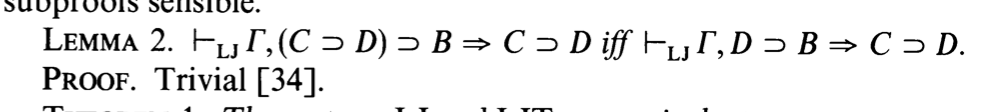
\includegraphics[width=0.95\textwidth]{Vorobieff-lemma}
\par\end{center}

\begin{center}
{[}R. Dyckhoff: \emph{Contraction-Free Sequent Calculi for Intuitionistic
Logic}, The Journal of Symbolic Logic, Vol. 57, No. 3 (1992), pp.
795-807{]}
\par\end{center}
\begin{itemize}
\item A stepping stone to this theorem:
\[
\left(\left(A\Rightarrow B\right)\Rightarrow C\right)\Rightarrow B\Rightarrow C
\]
Proof (obviously trivial):
\[
f\Rightarrow b\Rightarrow f\:(\_\Rightarrow b)
\]
\end{itemize}
\end{frame}

\begin{frame}{Making practical use of the CH correspondence}


\framesubtitle{Implications for actually writing code}

What can we do now?
\begin{itemize}
\item Given a fully parametric type, decide whether it can be implemented
in code (``type is inhabited''); if so, \emph{generate} the code
\item Let \texttt{curryhoward} fill in the code when it is trivial to do
so
\end{itemize}
What problems cannot be solved with these tools?
\begin{itemize}
\item Automatically generate code satisfying properties (e.g.\ isomorphism)
\begin{itemize}
\item The heuristics will help in some cases
\end{itemize}
\item Express complicated conditions via types (e.g.\ ``array is sorted'')
\begin{itemize}
\item Need dependent types for that (Coq, Agda, Idris, ...)
\end{itemize}
\end{itemize}
\end{frame}

\begin{frame}{Title, Abstract, Bibliography}

\begin{quotation}
Generating code with the Curry-Howard correspondence: Type inhabitation
at compile time
\end{quotation}
I implemented a library for compile-time code generation from Scala
type signatures. The library uses (compile-time) reflection, the Curry-Howard
correspondence, and a theorem prover for the constructive propositional
logic. Using this library, I illustrate how the Curry-Howard correspondence
maps types into propositions and proofs into code. I will also explain
some details of the algorithm I used for automatic code generation
from type signatures. As an illustration of using this library for
automatic code generation, I demonstrate working examples such as
implementing \texttt{\textcolor{blue}{\footnotesize{}map}} and \texttt{\textcolor{blue}{\footnotesize{}flatMap}}
for the Reader and State monads.
\end{frame}

\end{document}
